\section{Disassembly} \label{sec:existing-disassembly}
As discussed in Chapter \ref{sec-challenges}, one of the major difficulties in
disassembly is differentiating code and data. While some successful disassembly
tools exist on the market~\cite{hex2014ida,kvroustek2017retdec,ghidra,radare},
these tools inevitably have substantial false positives (take data as code) and
false negatives (ignore code as data). In this section, we mainly discuss
several state-of-the-art disassembly and binary rewriting techniques that
solved the problem to a large extent.

\subsection{Disassembly with Less Errors} \label{sec:existing-less-errors}
Bauman et al. proposed \textit{superset disassembly} that employs the brute force method to guarantee no false negatives~\cite{bauman2018superset}. Specifically, superset disassembly takes every offset in the text segment as one possible start of an instruction, called superset instruction. It finds intended sequences of instructions by brute force disassembling every possible instruction, although the bytes of adjacent instructions may overlap.
%
In this way, it can be guaranteed that there is no false positive in the result, and thus enabling error-free binary rewriting. However, the disassembled program will be bloated as lots of false-positive instructions exist. The bloated instructions could cause substantial size and runtime overhead because getting the instruction to be executed needs a table lookup each time, especially in practice, a binary writer based on superset disassembly has to instrument all superset instructions.
% probabilistic disassembly
Thus, Miller et al. proposed \textit{probabilistic disassembly} based on superset disassembly to reduce the number of false positives further~\cite{miller2019probabilistic}. Probabilistic disassembly aims to reason the inherent uncertainty in the binary analysis caused by the lack of debugging information. The basic idea is to compute the probabilities of each address being the true positive start of an instruction. They define three hints that imply true positive instructions and assign prior probabilities to these hints, then perform probabilistic inference to summarize the confidence of true positives from these evidence.

% Datalog disassembly
Besides the false negatives free but costly disassembly approaches, some research aims to disassembly faster while keeping a low false positives/negatives rate. Flores-Montoya et al. present \texttt{Ddisasm}~\cite{flores2020datalog}, a disassembly framework based on Datalog combining static analysis and heuristics, achieving lower false positives and false negatives rates compared with \texttt{Ramblr}~\cite{wang2017ramblr}. This framework takes advantage of Datalog, enabling faster empirical evaluation of new heuristics and analyses.
% XDA NDSS 2021 Suman Jana
In addition, \texttt{XDA} (Xfer-learning DisAssembler) leverages transfer learning to use different contextual dependencies learned from machine code for accurate disassembly~\cite{pei2020xda}. Although this framework surpasses SOTA disassemblers on both speed and accuracy, errors in results cannot be easily fixed without retraining, which prevents machine learning-based frameworks from being iteratively updated frequently. Also, it requires expensive GPUs to outpace existing tools on speed.

\subsection{Binary Rewriting} \label{sec:existing-symbolization}
% Uroboros
Even though we can get correct disassembly code, there is still a huge gap between achieving successful binary rewriting. This gap is summarized as the symbolization problem or relocatable problem~\cite{wang2015reassembleable,wang2017ramblr}, as discussed in \S~\ref{sec:challenges-symbol}. \texttt{Uroboros} was the first disassembler to be capable of not only disassembling code, but also symbol information from striped binaries automatically~\cite{wang2015reassembleable}. \F~\ref{fig:uroboros} illustrates c2c(code to code), c2d(code to data), d2d(data to data), and d2c(data to code), in total four types of symbol references defined in \texttt{Uroboros}. To solve the symbolization problem, \texttt{Uroboros} summarized several heuristics to distinguish these four types and thus successfully rewrote all \textsc{Coreutils}, \textsc{SPEC INT 2006}, and 7 real-world programs. More importantly, after correctly recovering symbol information, \texttt{Uroboros} is able to disassemble-reassemble iteration 1,000 times, in which the output of each iteration becomes the input of the next round, with almost zero code size explosion and speed slowdown.

\begin{figure}[tb]
  \centering
  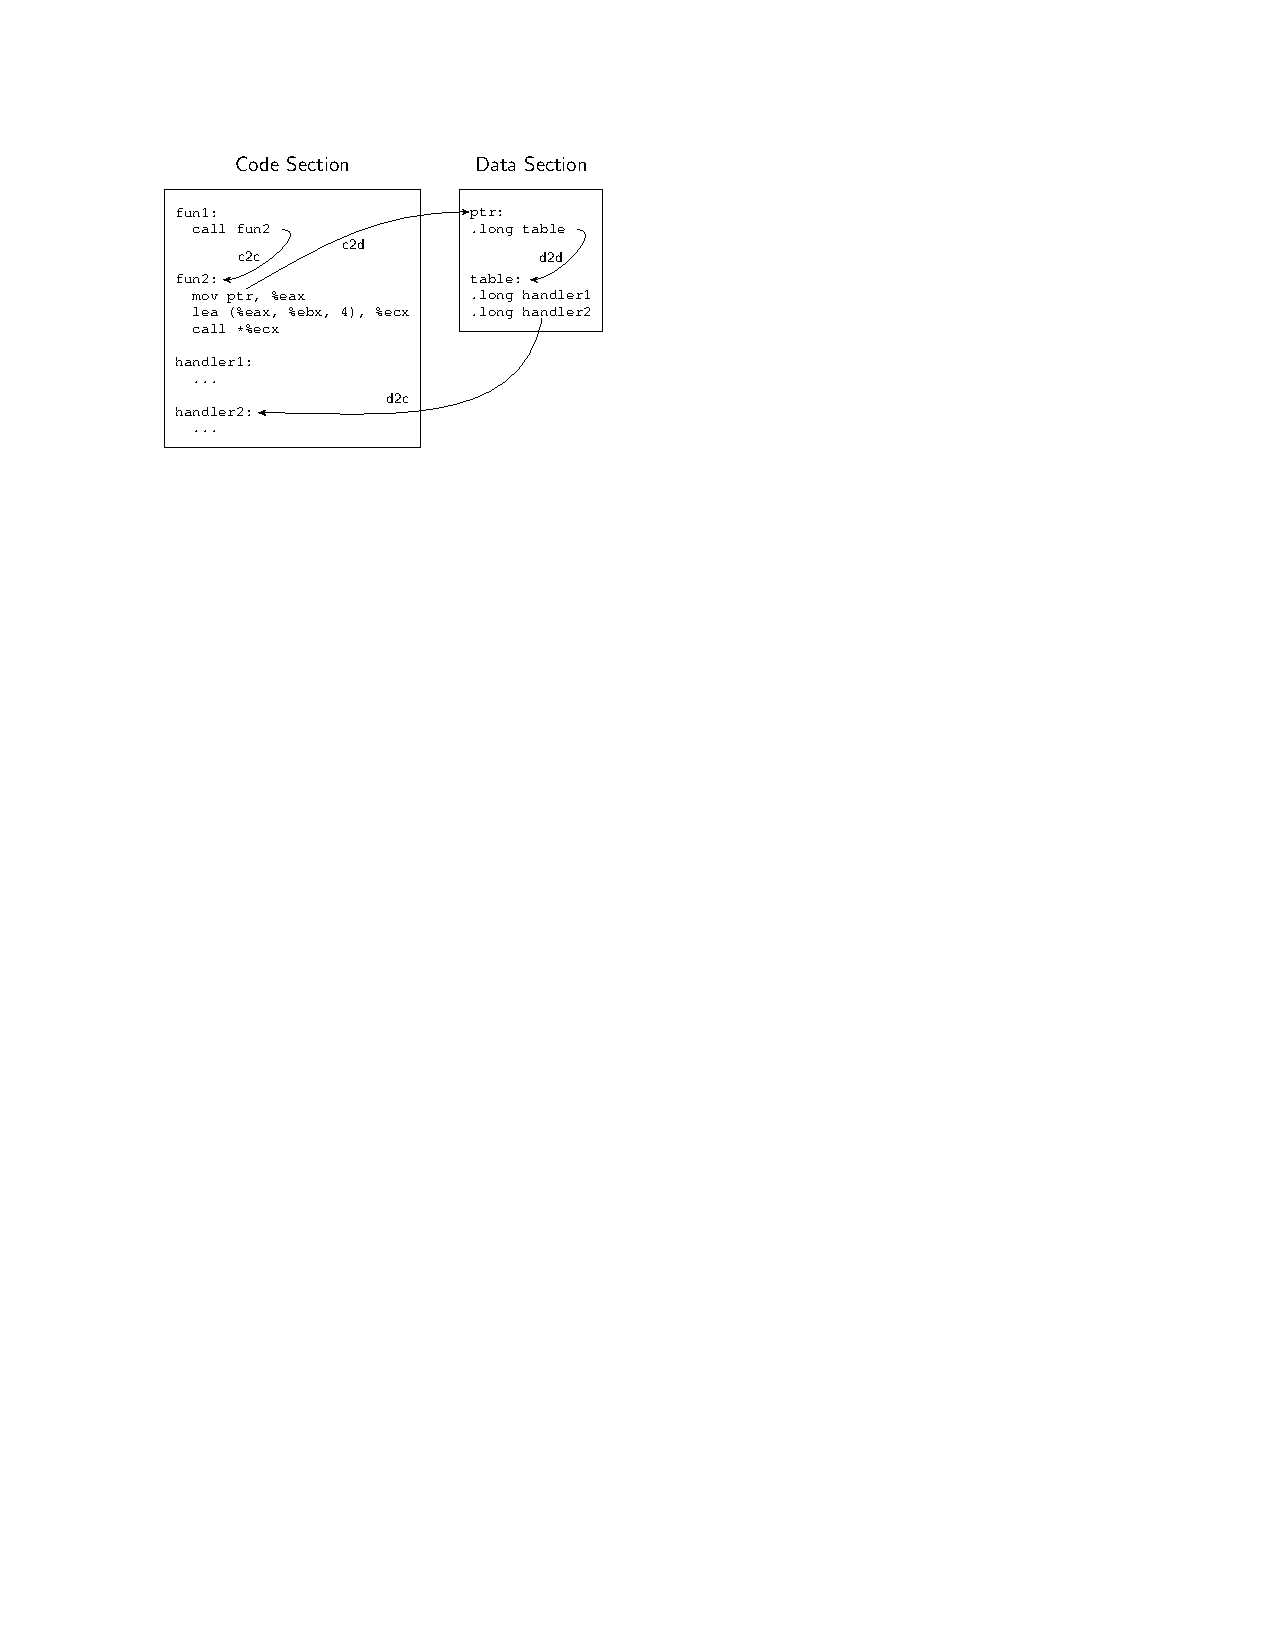
\includegraphics[width=0.6\textwidth]{fig/uroboros.pdf}
  \caption{Different types of symbol references in assembly code~\cite{wang2015reassembleable}.}
  \label{fig:uroboros}
\end{figure}

% Ramblr
However, manually designed heuristics can hardly achieve binary rewriting across compiler versions because of various optimization and code generation strategies.
\texttt{Ramblr} proposed more sophisticated heuristics and analyses for symbolization. Based on the \texttt{angr} binary analysis platform~\cite{shoshitaishvili2016sok}, \texttt{Ramblr} is able to rewrite all \textsc{Coreutils} programs and 143 binaries from the DARPA Cyber Grand Challenge (CGC) on newer compilers (\texttt{gcc} 5.4.1 and \texttt{Clang} 4.4) with more optimization levels (\texttt{O0}, \texttt{O1}, \texttt{O2}, \texttt{O3}, \texttt{Ofast}, and \texttt{Os}). Although Ramblr went further than the most advanced binary rewriting technique of the time, it did not go beyond the inherent limitations of heuristics and was still error-prone on higher versions of compilers.

\subsection{PIC Binary Rewriting} \label{sec:existing-pic}
Generally speaking, recovering symbol information from stripped binaries has to rely on complicated binary analysis or error-prone heuristics, and thus efficient and error-free static binary rewriting is difficult. With the trend of PIC (Position-Independent Code) becoming the default option of mainstream compilers, some of the subsequent research turns to narrow down their research scopes to 64-bit PIC code only to circumvent the challenging symbolization problem.
% RetroWrite
\texttt{RetroWrite} designed a principled symbolization strategy without heuristics~\cite{dinesh2020retrowrite}. \texttt{RetroWrite} leverages relocation information existing in PIC binaries to identify symbolizable constants. More specifically, it recovers symbols by
\begin{itemize}
  \item[1)] converting targets of control-flow instructions (i.e., calls and jumps) to symbols (recovering code-to-code references),
  \item[2)] converting the PC-relative addresses to symbols (recovering code-to-code and code-to-data references) to further complete the control flow graph, and
  \item[3)] converting data relocations to symbols (recovering data-to-data and data-to-code references).
\end{itemize}

In this way, \texttt{RetroWrite} presented a sound and scalable symbolization approach, which makes it robust enough to support multiple security-critical downstream applications, such as \texttt{AddressSanitizer}~\cite{serebryany2012addresssanitizer} and coverage-guided greybox fuzzing~\cite{zalewski2014american}.

% Egalito
Similarly, \texttt{Egalito} uses the relocation information that exists in x86-64 and ARM64 binaries to tackle the symbolization problem. Egalito first lifts disassembled code into the machine-specific, layout-agnostic Egalito IR, then identifies code pointers and reconstructs jump tables on the IR, thus theoretically enabling cross-platform binary rewriting. Their evaluation shows that \texttt{Egalito} is adequate to augment hardware/compiler deployment with multiple defense techniques, including a retpoline defense against Spectre ~\cite{kocher2019spectre}, a software implementation of Intel’s CET~\cite{cet}, and a continuous code randomization defense named JIT-Shuffling~\cite{williams2016shuffler}.

\subsection{Others} \label{sec:existing-dis-others}

\begin{figure}[tb]
  \centering
  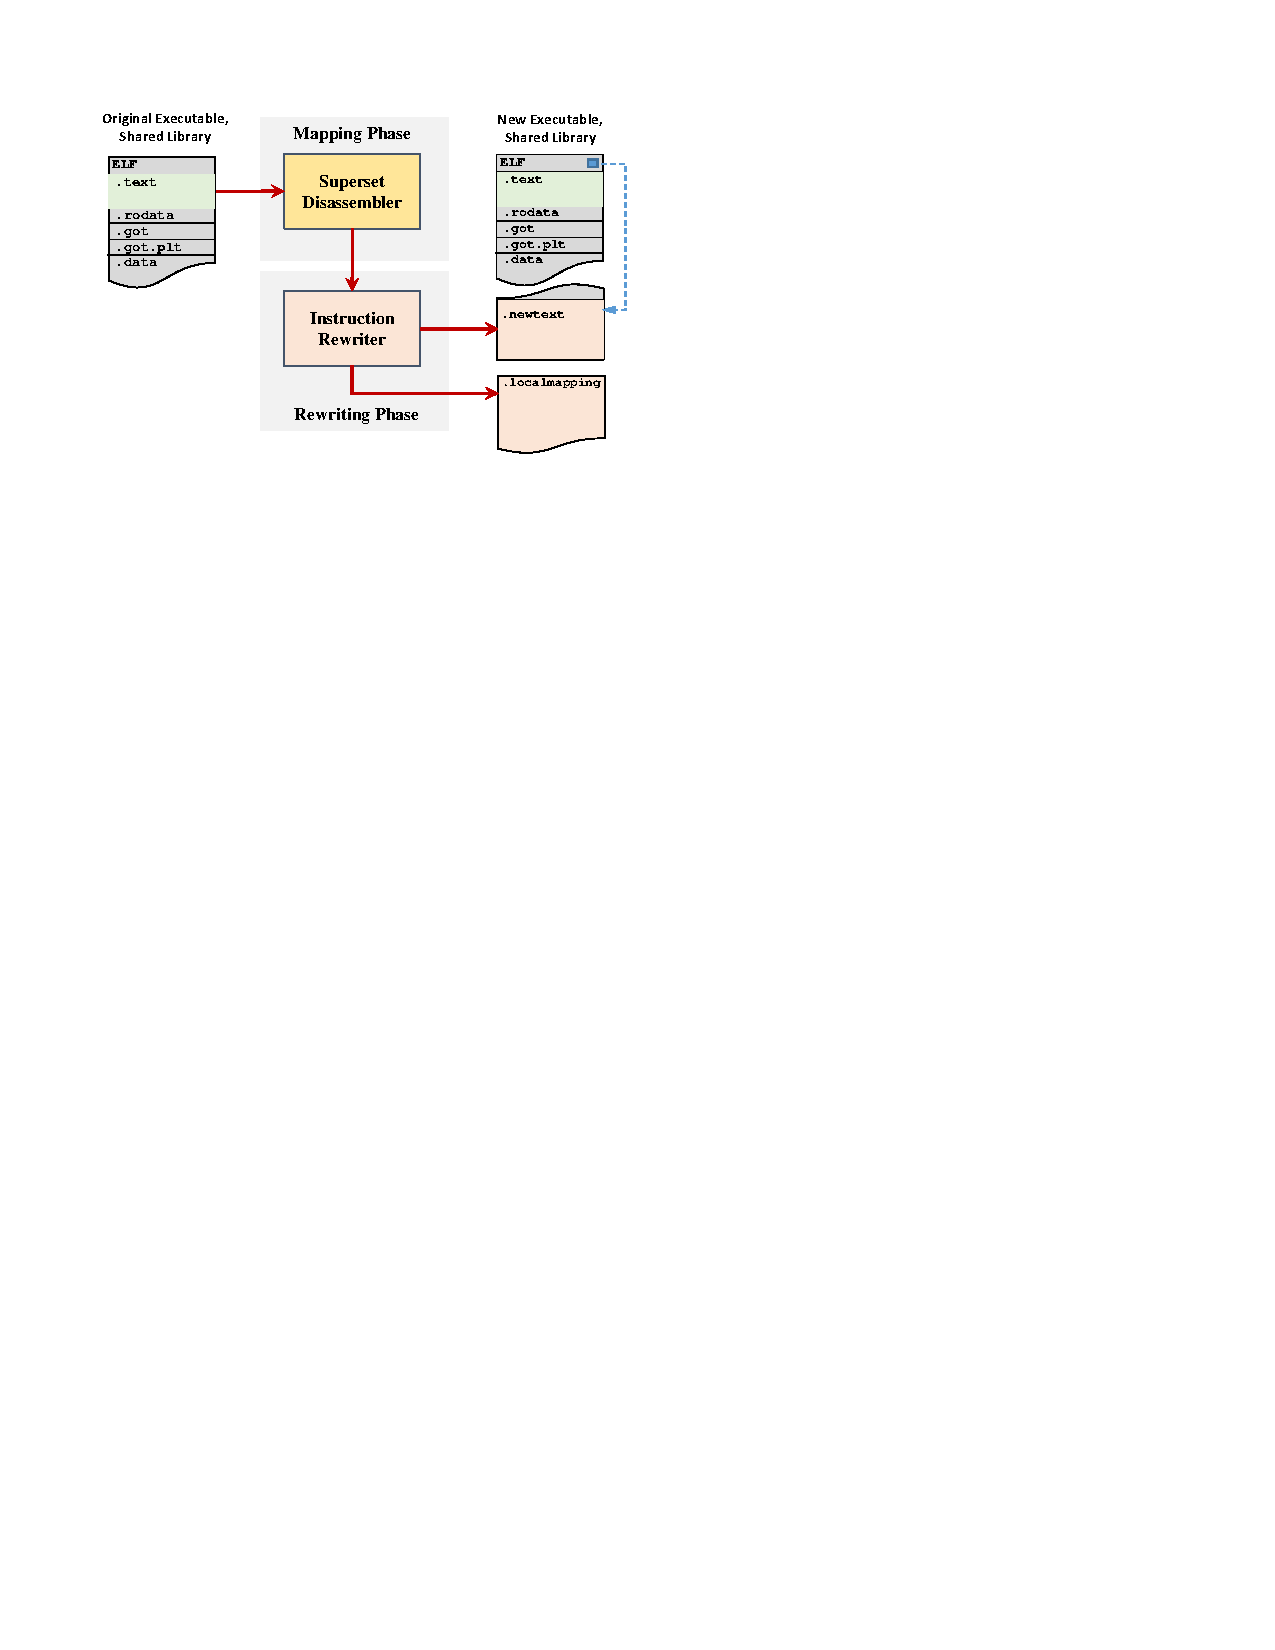
\includegraphics[width=0.6\textwidth]{fig/superset.pdf}
  \caption{Overview of \textsc{Multiverse}~\cite{bauman2018superset}.}
  \label{fig:superset}
\end{figure}

% Superset / Probabilistic disassembly way
Except for recovering symbol information precisely, another line of research tries to sacrifice code size and performance for stable binary rewriting. For example, \textsc{Multiverse}~\cite{bauman2018superset,miller2019probabilistic} appends the disassembled code and a mapping from old addresses to new addresses after the original binary as the \texttt{.newtext} segment and \texttt{.localmapping} segment, as illustrated in \F~\ref{fig:superset}. The original \texttt{.text} segment is kept as read-only data so that recompiled elf binary could read function pointers (code-to-code and data-to-code references) from it and translate the pointers to its new address by looking up the \texttt{.localmapping} segment.

% E9Patch
On the other hand, \textsc{E9Patch} introduced a new idea to achieve binary rewriting without control flow recovery~\cite{duck2020binary}. For the purpose of more flexible static x86-64 binary rewriting, \textsc{E9Patch} came up with a set of instruction-level rewriting methodologies that can insert jumps to trampolines while not changing the layout of the original program. Since this approach does not need a control-flow graph or any binary analysis, it can be easily applied to large-scale binaries.
%
\F~\ref{fig:e9patch} illustrates one trampoline example of \textsc{E9Patch}. The original instruction, \texttt{mov \%rax,(\%rbx)}, corresponds to the bytes sequence \texttt{48 03 48}, \textsc{E9Patch} only modify the first 3 bytes to change the instruction to a \texttt{jmpq} instruction. The target of this \texttt{jmpq} instruction is restricted to a small memory region (\texttt{0x8348XXXX}), where the instrumented code could be placed. The \textsc{E9Patch} approach is robust as no heuristics are used. However, it is still limited as not all x86 instructions could be leveraged with their techniques. According to the evaluation results, this approach could achieve around 99\% probability of successful instrumentation.

\begin{figure}[tb]
  \centering
  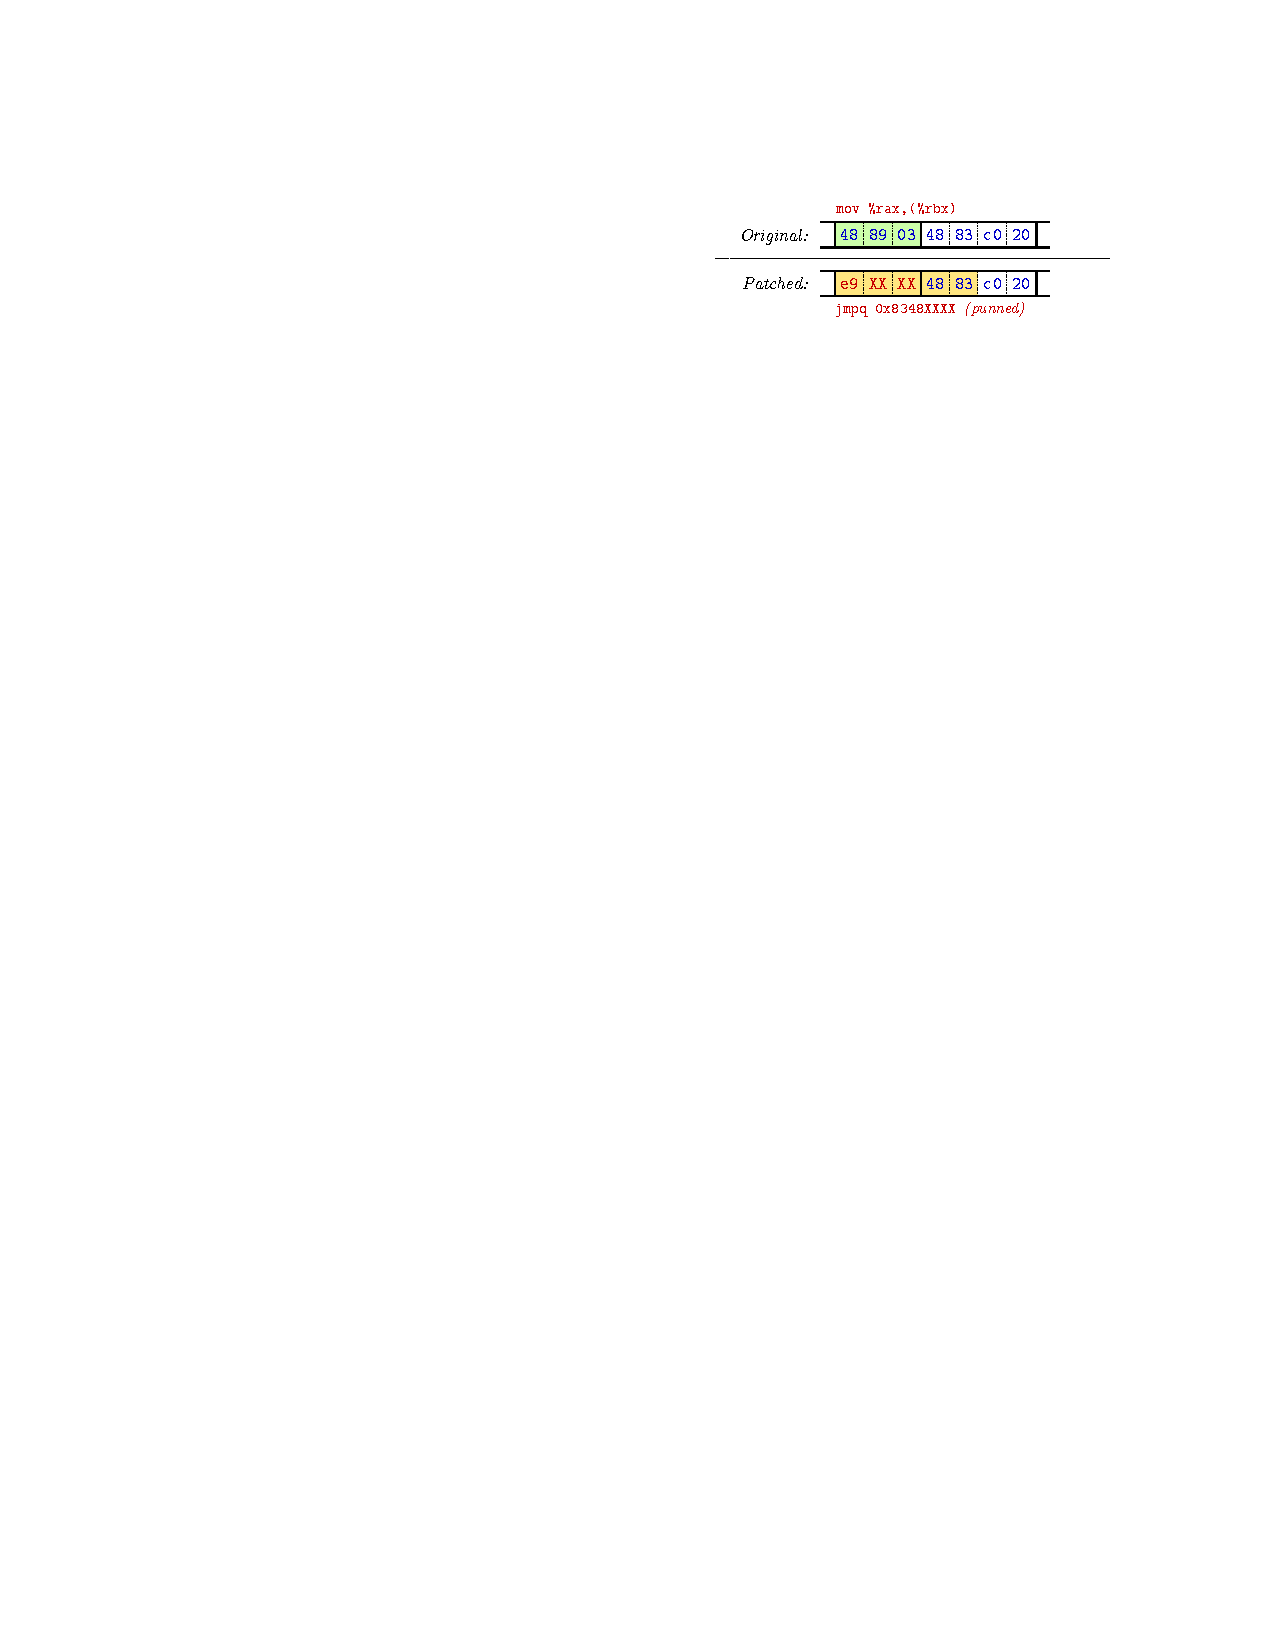
\includegraphics[width=0.6\textwidth]{fig/E9Patch.pdf}
  \caption{Illustration of \textsc{E9Patch} trampoline~\cite{duck2020binary}.}
  \label{fig:e9patch}
\end{figure}

% StochFuzz
In addition to all the static methods discussed above, one recent research proposed an interesting idea, \textsc{StochFuzz}, that solves the symbolization problem dynamically~\cite{zhang2021stochfuzz}. While admitting the difficulties that exist in control flow recovery and symbolization process, this approach does not try to design complicated analyses or heuristics. Instead, it accomplishes symbolization based on observations of runtime behavior, i.e., it dynamically verifies whether an address corresponds to data or code.

\begin{figure}[tb]
  \centering
  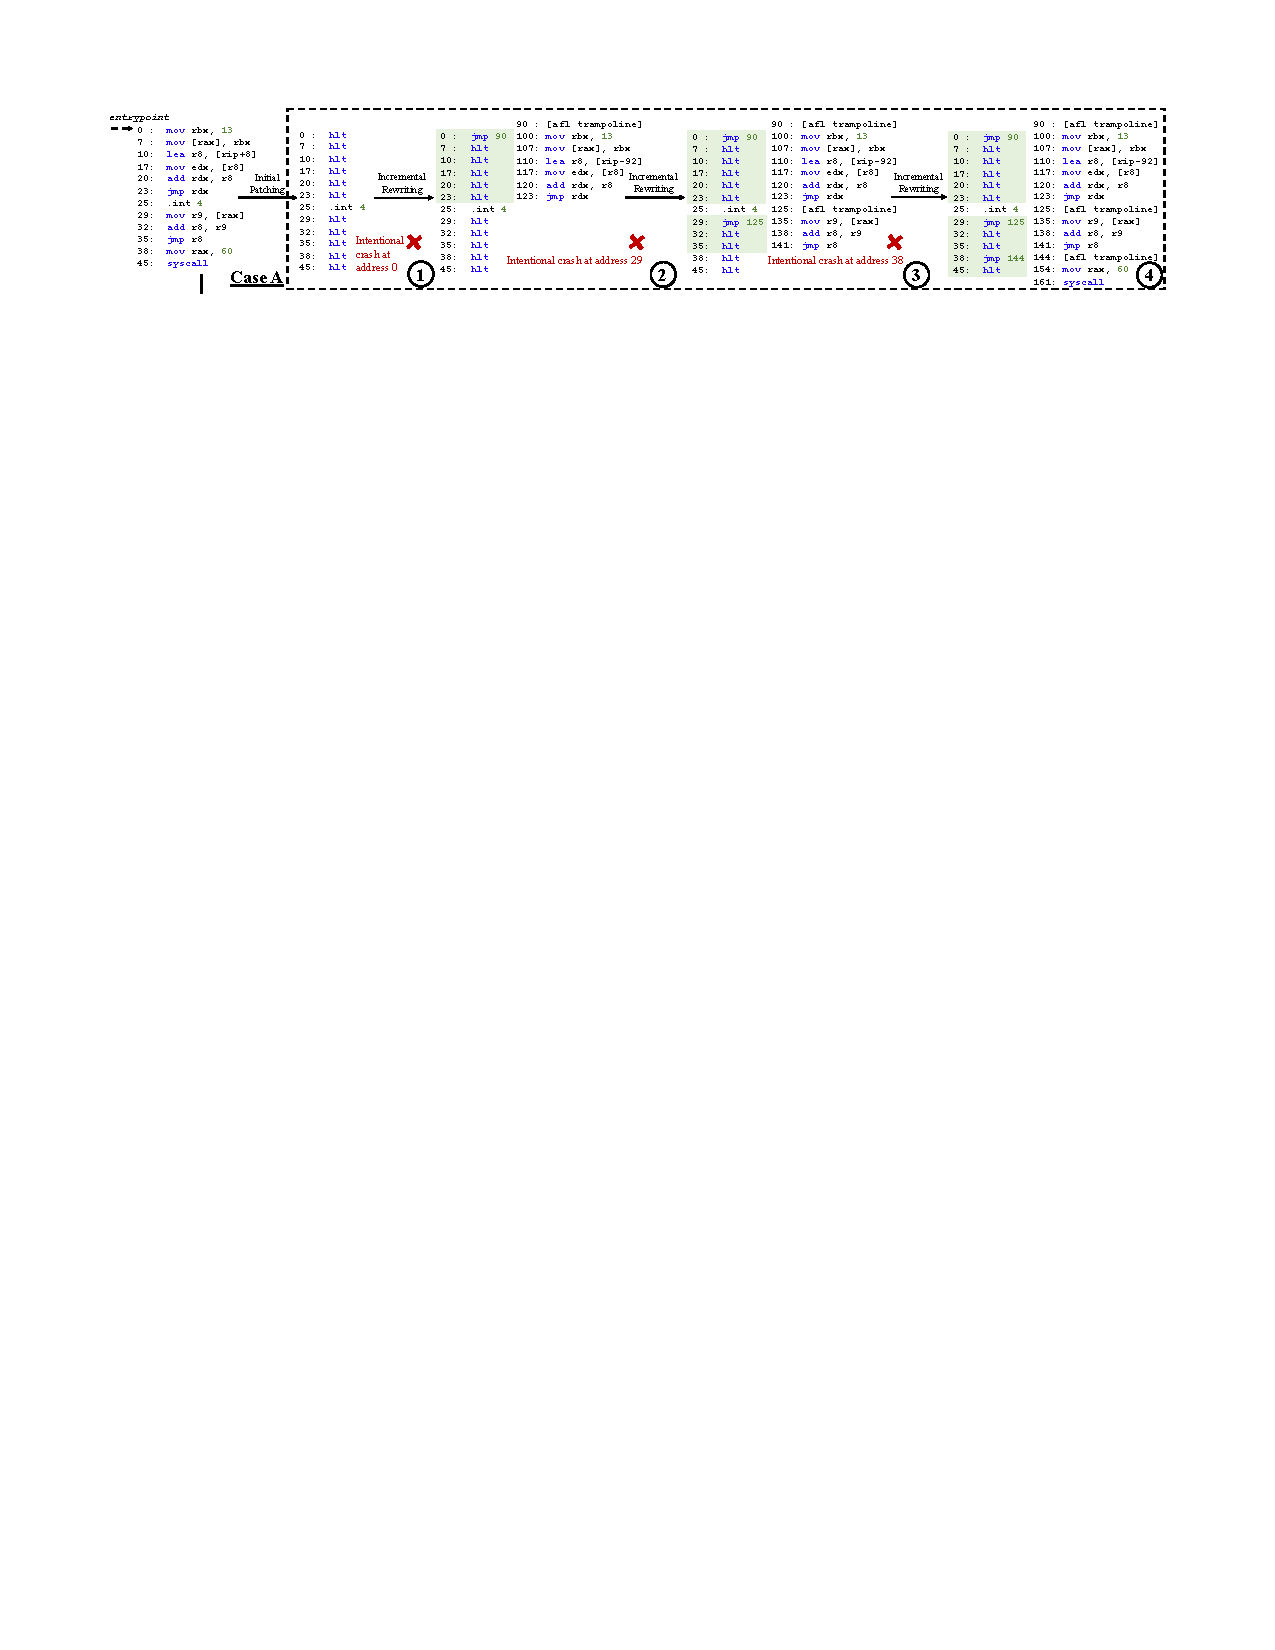
\includegraphics[width=1.0\textwidth]{fig/STOCHFUZZ.pdf}
  \caption{One example of \textsc{StochFuzz} rewriting strategies~\cite{zhang2021stochfuzz}.}
  \label{fig:stochfuzz}
\end{figure}

To be more specific, this approach proposes an incremental and stochastic rewriting technique that leverages the fuzzing technique to validate assumptions about symbols. It generates many different versions of rewritten binaries then tries to trigger specific behavior with fuzzing runs.
%
\F~\ref{fig:stochfuzz} illustrate one of the rewriting strategies used in \textsc{StochFuzz}. Given the program listed, the code will be first replace with \texttt{hlt} instruction which will case a segment fault, as shown in \textcircled{\raisebox{-0.9pt}{1}}. The segment faults, called \textit{intentional crashes}, indicate that a code block that was not disassembled was found. \textsc{SotchFuzz} starts by fuzzing the rewritten binary. Once the segment fault occurs, the code block that starts from the current address will be disassembled and placed at a \textit{shadow space} marked as a afl trampoline in the figure. (Note that the instruction at address 110 is \texttt{lea r8, [rip - 92]}, in which \texttt{rip - 92} corresponds to the original code address \texttt{rip + 8}.) After the disassembling, the new binary will be compiled and fuzzed again. Overall, this binary is recompiled with one \textit{incremental} block of disassembled code each time. Therefore this process is called ``incremental rewriting''. Eventually, all covered blocks will be correctly disassembled by iteratively rewriting and fuzzing without ``data or code'' confusion.
